\section{Overview}

In the last few decades we have learned that the brain does not process all incoming sensory information equally. According to our goals and context we filter out irrelevant information and select for sensory inputs that are important. At first, the idea that this filtering occurred in sensory cortex was a surprise-- but it is now generally accepted that changes in sensory representation drive selection.

In this thesis, I investigated the processes underlying selective visual attention in the human cortex. The overarching goal was to establish how information is selected from visual representations for use during adaptable behavior. To do this, I started by extending an existing linking model of contrast, which controls the visibility of images, to a second feature: coherence. These two ways of manipulating the visibility of motion required a new framework to be built, demonstrating how visual cortex is sensitive to each of these features and whether they interact. I then connected this framework to perception and tested different hypotheses about how that link might work by building computational linking models. Those models revealed that the scale of sensory changes due to attention were insufficient to capture perception. We expect these results to hold true for other forms of selection, e.g. by spatial location, color, or motion direction, and sought to demonstrate this in the final section of the thesis.

\subsection{Aim 1: Using linking models to compare implementations of selective visual attention}

The prevailing view is that attention is implemented by modifications of sensory responses. But without a computational linking model it is impossible to know whether these sensory changes are the only changes occurring during selective visual attention. 

\textbf{In Chapter 2, I build a quantitative framework for two features of motion visibility.} Contrast and motion coherence both control the visibility of motion and their representations in human visual cortex are similar. This makes them excellent tools to study whether sensory change alone can account for the behavioral effects of attention. In this chapter, I measure and quantify how these features are represented to lay the ground work for a linking model.

\textbf{In Chapter 3, I use a linking model to show that sensory change is insufficient to account for all the behavioral effects of attention.} I first validate that a linking of motion visibility can be constructed, based on the quantitative framework developed in Chapter 2. Then, using the validated linking model I show that the sensory change occurring during selective visual attention is insufficient to account for behavioral changes -- a flexible readout must be a necessary component.

\subsection{Aim 2: Comparing different forms of sensory selection on a shared perceptual metric}

One question we asked ourselves after completing Aim 1 was whether our results would be consistent in other features. Is selection by motion visibility similar to selection by spatial location, by color, or by motion direction? Although we know that different visual features are processed in different ways, this does not necessarily mean that selection by these features requires different computational resources and implementations.

\textbf{In Chapter 4, I address this aim by building a psychophysics experiment with which I compare the strength of spatial and feature-based attention on a common metric.} I demonstrate in these experiments that the sensitivity (i.e. the variability in response error) is constant across different forms of selection. 

\subsection{Aim 3: Extending our findings to selection by location, color, and motion direction}

The results of Aim 2 suggest that all forms of selection share a similar algorithm while the results of Aim 1 suggest that a large part of this process occurs outside of sensory cortex. \textbf{In Chapter 5}, I introduce an experimental paradigm that we are using to explore whether this can be demonstrated for features other than motion visibility. In this paradigm we build a stimulus that can be selected by spatial location, by color, or by direction of motion.

\break

Before going into detail about my experiments and computational models, I will introduce these topics briefly by reviewing what is known about selective visual attention. In particular, I will focus on the history of how selection might be implemented as a computation in the human brain. Examples will be drawn from the existing literature on selection by spatial location, color, motion direction, and higher order features such as faces or people. I will also discuss the origin and existing uses of computational linking models.

\section{Sensory selection}

** new outline **

what is sensory selection?

what is the history of sensory selection research?

how might sensory selection be implemented

organization of visual cortex

measurements of sensory selection

models of sensory selection

limitations to existing models of sensory selection

using computational linking models to correctly characterize the scale of sensory selection in cortex

* examples of selection by contrast
* selection by color
* selection by location
* selection by motion direction



We all know, more or less intuitively, what it is like to attend to something that we see. When stopped at an intersection, a driver might be motivated by their context to focus on the direction of nearby cars, the movement of pedestrians, and the stop signs or traffic lights in their vicinity (Fig. \ref{fig:c0f1}). The ease with which we can deploy attention hides a complex set of changes which occur inside the brain and which change our sensory perceptions. By moving such experiences into the laboratory we can operationalize them (Fig. \ref{fig:c0f1}b). That is to say, we can break down a complex process such as attention into the discrete changes which result from it. For example, attention might improve reaction times, detection, or the ability to discriminate between stimuli, but not necessarily all of these and not necessarily all to an equal extent. Once operationalized, we can begin to track these back to their roots inside of the brain. As an example, one of the earliest findings in sensory selection research was that information to which we direct our focus is enhanced, slightly, at a huge cost to information which we ignore. 

\begin{figure}[ht]
\centering
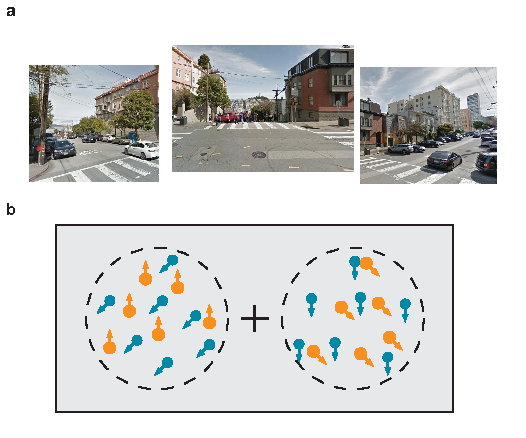
\includegraphics[keepaspectratio,width=0.75\textwidth]{figs_c0/task_example.pdf}
\caption[Selective visual attention tasks]{Natural and operationalized tasks which engage selective visual attention. (a) A driver, stopped at an intersection, puts more contextual weight on information such as the direction of nearby cars, the movement of pedestrians, and stop signs or traffic lights in their vicinity. While those features of the visual environment might be enhanced irrelevant information, like the colors of the sky or houses, might be filtered out. (b) To operationalize selective visual attention the task must be simplified to a form which has parameters. Here the color of the dot patches can be used to select out two dot patches. Later, an observer could be asked to recall the motion direction of the selected patches. An alternative way of selecting information from the same scene would be to select the two overlapping patches on the same side. In both cases, the color, motion direction, stimulus duration, and visibility can all be manipulated to change the difficulty of the task. Having such parameters is essential to be able to build computational linking models}
\label{fig:c0f1}
\end{figure}

One of the earliest results in attention research was the fact that perceptions become more "intense" or "clear" when focused upon, the result of careful introspection into the experimenter's own conscious experiences \citep{Helmholtz1924-rl,James1981-cj,Kuelpe1902-qz,Titchener1908-bx}. These intuitions were not without merit, as spatial attention to some stimuli does appear to lead to a change in the appearance of a stimulus \citep{Carrasco2018-sb}. In fact, when carefully measured, these enhancements come at a cost. Perhaps the earliest example of this is a set of experiments in which observers were asked to echo speech from one ear at a time \citep{Cherry1953-as}. The transition from introspection to ‘objective’ measurement can be highlighted in the way these experiments were introduced, quoting from \citet{Cherry1953-as}: ``the `subject' under test (the listener) is regarded as a transducer whose responses are observed when various stimuli are applied, whereas his subjective impressions are taken to be of minor importance''. This approach was effective. The field made an abrupt move toward understanding sensory systems as processing units. Any given stimulus could be processed in a serial or parallel manner and processing might go to `completion' or be halted at a certain point. Measuring the knowledge of a subject about an attended or ignored stimulus therefore assesses the extent of processing which has occurred for that stimulus. For example, for the echoing task described above, an observer might be asked whether they had retained knowledge about an un-echoed (and therefore, unattended) voice. If they could recall simple low-level features, e.g. that the speaker had a higher-pitched voice, then a researcher could conclude that parallel processing of both streams had occurred up to pitch processing [cite?]. They could then also conclude that processing of the ignored stimulus had then been halted, before the point of complete semantic understanding. Such results led researchers to begin to distinguish between stages of processing: an early parallel stage in which incoming sensory information is processed without immediate limits in capacity, and a second limited capacity serial stage from which complex decisions could be made.

Several early theories of attention focused on when selection occurs relative to the parallel and serial stages of processing. These theories fell out of the observations made above, that some features of auditory, as well as other sensory, stimuli are available for decision making regardless of the observers focus while other features must be attended to be available. To reconcile these facts researchers suggested a bottleneck and proposed that this was the mechanistic implementation of selective attention. The first such modern theory was Broadbent’s Filter theory \citep{Broadbent1958-ny}, which included an early bottleneck. In Filter theory visual information is processed in parallel until low-level features (location, intensity, frequency) are resolved. At this point, parallel processing gives way to a serial ‘complete’ processing of object identity, form, etc. The alternative theory, late selection, suggests that processing occurs up to semantics in an unconscious parallel manner \citep{Deutsch1963-ac}. An example best illustrates the distinctions in these theories. Again, if an observer is echoing one speaker while ignoring a second, a late selection account predicts that a substantial amount of information is nevertheless available about the ignored voice. This is because late selection predicts that a semantic-level processing of speech will occur regardless of sensory selection, leaving high-level information available to an observer. Evidence for this comes from experiments in which observers orient to highly salient, but also very high-level features, such as their own name, even when focused on other tasks \citep{Moray1959-fn}. This suggests that not also features are processed in identical ways. Selection theories were expanded upon, based on this suggestion that features might differ in their form of processing and not be consistently selected out in one step. Instead, it was suggested that features might be attenuated \citep{Treisman1960-qs} or that selection might be limited by variable capacity at different stages of processing \citep{Kahneman1973-af}.

Selective attention has been most heavily studied in the visual domain, in part because of the close relationship between selecting information in the world and orienting of the eyes. Spatial orienting can occur both in an overt movement of the eyes, but also covertly without eye movements. This covert attention accelerates responses \citep{Eriksen1972-qj,Posner1980-cr} and both improves detection performance and increases discrimination sensitivity \citep{Carrasco2011-xp}. Cues about important locations can both be imposed externally on an observer \citep{Posner1980-wb} or the result of internal guiding of attention toward the cued location. Covert attention be either spatial, related to eye movements, or featural \citep{Rossi1995-wa} as described below for search tasks. Because of this close relationship between selection with eye movements and vision, researchers have focused in particular on the implementation of selective attention in the visual system. 

\section{Implementations of selective visual attention}

Selective attention is a balancing act for the brain, which must weigh the possibility of needing unattended information against the strength of sensory selection. In an early selection theory, information is being thrown out before complete processing -- which could be potentially disadvantageous if that stimulus later becomes important for behavior \citep{Mack1998-nq}. Late 20th century research on attention was well aware of this fact, and researchers showed that in different contexts sensory selection can be more or less complete at filtering out irrelevant information. In a few particularly dramatic demonstrations \citep{Haines1991-si,Mack1998-nq,Neisser1979-mm,Simons1999-ng} observers can be shown to entirely lose access to otherwise highly salient information, but only when performing a task with significant cognitive load \citep{Lavie2005-aw,Lavie2004-ub,Rees1997-hd}. In vision, like in audition \citep{Moray1959-fn}, some visual information is processed no matter what, as scene gist can survive inattention, perceptually \citep{Li2002-ji} and as decodable information from measurements of BOLD signal in visual cortex \citep{Peelen2009-us}. These examples highlight the delicate balance that the brain must maintain: with limited resources how should the brain allocate these to efficiently sample the sensory world? Early research on the implementation of attention put this question to the side while first exploring the possible effects of attention on sensory processing. In apparent contradiction with the specific bottlenecks proposed by early and late selection theories, physiologists found that behavioral selection results in neural changes throughout the brain: in early visual cortex (where, presumably `parallel' processing occurs), higher visual cortex, and in non-sensory regions. Reconciling these observations with the behavioral effects of selective attention has become a major goal of cognitive neuroscience. 

Modern neuroscience now deploys a multitude of neural recording techniques to understand how behavioral selection might be implemented by the brain. Both at a coarse scale in humans and at the level of individual neurons in primates and, very recently, rodents. In humans and non-human primates attention has been shown to alter the response gain of neurons in the visual system, including in the LGN \citep{OConnor2002-mx}, in V1 \citep{Motter1993-av}, V2 \citep{Buffalo2010-lr,Luck1997-sq,Motter1993-av}, V3 \citep{Liu2007-jx,Pestilli2011-gi,Saenz2002-fs,Silver2007-vd}, V4 \citep{Buffalo2010-lr,Connor1996-nm,Luck1997-sq,McAdams1999-jy,Moran1985-cv,Motter1993-av,Reynolds2000-mg,Spitzer1988-ib}, V3A \citep{Serences2007-le},  MT \citep{Beauchamp1997-rh,OCraven1997-ej,Saenz2002-fs,Seidemann1999-oz,Serences2007-le,Treue1999-mp,Treue1996-ez} and MST \citep{OCraven1997-ej,Treue1996-ez}, and in IT cortex \citep{Chelazzi1998-gx,Moran1985-cv}. Using BOLD imaging these changes can be observed simultaneously throughout almost all of early visual cortex \citep{Liu2007-jx,Pestilli2011-gi,Saenz2002-fs,Silver2007-vd} and ventral temporal cortex \citep{Baldauf2014-uj}. Although the neurochemical mechanisms of these effects remain unclear, muscarinic acetylcholine receptors are known to play a key role \citep{Herrero2008-am}. Changes to sensory representations occur both for spatial attention tasks \citep{Klein2014-oe,McAdams1999-jy,Mitchell2009-do,Pestilli2011-gi,Womelsdorf2006-np} and feature-based attention tasks \citep{Baldauf2014-uj,Harel2014-wd,Huk2000-uj,Jehee2011-mb,Saenz2002-fs,Saenz2003-qz,Serences2007-le,Treue1999-mp}.

Measurements of physiology have confirmed that not all visual properties are processed in an equal manner. Behavioral results predicted this \citep{Li2002-ji,Moray1959-fn} and the theories outlined above make those hypotheses explicit. One of the easiest operationalized tasks in which to observe this is during search \citep{Wolfe1994-ew}. In a search task, an observer will be cued in advance to reveal the location of a particular item, e.g. by pointing to it, or to assess its presence, e.g. by pressing a button to indicate that it is present. The item will be hidden among a set of distractors whose properties determine the difficulty of the task. Such tasks are trivial when the target stimulus differs from the distractors along certain key dimensions: color, orientation, spatial frequency. Trivial, in this case, means that the processing required to solve the task occurs in parallel and the solution is found by the observer in “one step”, so to speak. This matches with experiments in the early visual system which show that neurons are characterized by their tuning to orientation, spatial frequency, and to particular regions of visual space \citep{Barlow1957-by,Hubel1962-pn}. The tiling of these neurons across retinotopic space results in visual field maps, of which there are more than a dozen identified in human visual cortex \citep{Wade2002-tt,Wandell2007-pr,Wandell2011-td}. In these simple search tasks, it appears that early visual cortex performs computations largely in parallel across these maps. Differences in the strength of signals across these maps, for each feature, can then result in ‘pop out’ of the relevant stimulus \citep{Nothdurft1993-xt,Treisman1985-dr}. 

Difficult search tasks involve conjunctions of stimulus properties \citep{Egeth1984-ch} which require attention to be directed in a serial manner to each item \citep{Treisman1980-gu}. The results from search experiments match the findings of early physiology experiments \citep{Hubel1959-fo,Hubel1968-na} which showed that the early visual cortex starts by processing in parallel some of the same simple features which `pop out' during search. Sharp differences in these features drive bottom-up attention, or salience, in which features that differ from their neighbors can cause an observer to orient to them. In contrast to this parallel stage, higher areas in visual cortex process complex stimuli such as objects, but this processing does not appear to occur in parallel for multiple objects. Instead objects trade off for representation according to the focus of attention \citep{Desimone1998-wf}. Instead of the repetitive receptive field structure in early visual cortex these areas have large receptive fields and retinotopic biases. These may be shaped by experience, for example there is a foveal bias in areas selective for faces and a peripheral bias in areas that are selective for locations \citep{Levy2001-oe}. Importantly, the physiological effects of selective attention are not isolated to any one of these areas. 

Our understanding of the neural implementation has advanced dramatically thanks to recordings of neuronal populations from animal models. But animal models have also held back research in important ways. In general it is not possible to probe an animals memory about unattended stimuli, rendering many classic psychophysics paradigms difficult to interpret. Whether the implementation of attention in a primate trained over months is similar to that in a human trained over the course of minutes is an unknown at the moment. Recently, mice have been shown to be able to exhibit selective attention \citep{McBride2019-py,Wang2018-ge}. This is promising for understanding the role of different brain areas in attentional selection, but also concerning. The mice in these studies exhibit a bias which resembles selective attention, but they also have high lapse rates compared to human observers. One explanation is that mice continue to explore the experiment space \citep{Pisupati2019-cl} whereas humans who learn from rules do not. Correctly taking these differences into account, perhaps by linking animal research directly to parallel human research, has a good chance of overcoming these issues. 

Despite the many results showing that sensory representations change during directed attention researchers have yet to converge on a consistent algorithm which implements selection. Instead, a number of competing theories exist for how sensory selection might proceed, including changes in sensitivity \citep{Reynolds2000-mg,Serences2007-le,Snyder2018-yr,Treue1999-mp}, shifts in feature selectivity \citep{Cukur2013-gx,David2008-zx,Kastner1998-bi,Klein2014-oe,Spitzer1988-ib,Womelsdorf2006-np,Womelsdorf2008-bm}, increases in baseline response \citep{Buracas2007-pe,Chen2012-fu,Fang2008-ny,Kastner1999-qu,Li2008-fe}, and changes in the structure of stimulus-driven and noise correlations \citep{Cohen2009-bt,Mitchell2009-do, Ruff2016-dv,Verhoef2017-cm}. All of these changes affect the information present in sensory cortex to different degrees. Depending on the overlap and correlation between stimulus representations enhancement to one stimulus may results in loss of (TODO: fix). In contrast with these theories, flexible readout which leaves stimulus representation unchanged \citep{Birman_undated-vk} may be a useful alternative when behavior needs to remain adaptable. Deciphering the balance of sensory change against change in readout requires models which can quantify the extent to which neural changes result in behavioral changes. 

\subsection{Computational linking models}

Measurements of the neural effects of selective attention are not sufficient to understand its implementation, they must be linked correctly to behavior. To reconcile changes in cortical activity with behavior, cognitive neuroscientists can link measurements of neuronal activity and behavior using computational linking models. One assumption underlying much of cognitive neuroscience is that when we make a measurement of cortical activity, we are seeing the same signals that the brain uses the solve sensory decision making. This is only an assumption; it is possible that sensory decision making (and other forms of neural processing) are based on subsets of signals, or population codes, which remain harder to measure. To avoid making errors in inference it is important to make these hypotheses (or assumptions) about implementation explicit in a form which can be tested against other possible hypotheses. One way to do this is to build computational models which lay out the steps from sensory signal to sensory decision. We refer to these as “linking models”, as they link together perceptual measurements and cortical ones. 

Recent work has begun to explore computational models which link measures of behavior to neuronal recordings, i.e. building linking models \citep{Barlow1972-kz,Brindley1960-gq,Cohen2010-xs,Newsome1989-fr,Pestilli2011-gi} (TODO: Cook & Maunsell, 2002). These experiments have shown that sensory responses are enhanced during directed attention while noise unrelated to the stimulus is altered and reduced \citep{Ecker2016-ro,Rabinowitz2015-uz,Snyder2018-yr}, which may be sufficient to cause neural activity to ``align'' to the dimension of readout \citep{Ruff2018-yx}. In human research similar tasks have been shown to cause estimates of receptive fields to shift \citep{Klein2014-oe} which might be sufficient to enhance spatial sensitivity at attended locations \citep{Klein2016-ox,Vo2017-oi} consistent with a response gain occurring in earlier layers of the visual system \citep{Baruch2014-gy,Miconi2016-ip}.
 
In a recent paper \citet{Pestilli2011-gi} found that a simple linking model of response gain during spatial attention was quantitatively insufficient to explain behavior. In that work, the authors found that a different form of readout was necessary to explain how the seemingly small changes in sensory representation could lead to large improvements in perceptual sensitivity. In non-human primates, linking models have been used to hypothesize about the possible roles of single neurons or populations in sensory decision making \citep{Newsome1989-fr}. Similar results in humans have implicated early visual cortex as a source of information about contrast discrimination \citep{Boynton1999-jd}. Finally, hypotheses about how sensory selection might alter the population code in cortex have been tested with linking models as well \citep{Cohen2011-pa}. Although none of these examples involve causal manipulations (although they often depend on the results of such research) they nevertheless have considerable value to the field because they make explicit their assumptions about how sensory decision making proceeds.

Linking models have the additional advantage that they allow researchers to begin to speculate about why sensory selection might be implemented in different ways. Depending on where sensory information is represented selection may have to occur in different ways: scene gist, which survives inattention \citep{Li2002-ji,Peelen2009-us}, may require very different kinds of selection to suppress compared to irrelevant spatial information \citep{Pestilli2011-gi}. Task demands likely also change the form of selection, as well as the computational costs associated with different cortical implementations (Gardner, 2019). Changing sensory representations during selective attention may reflect a computationally efficient solution where the visual system is discarding, and therefore not fully processing, stimuli that are irrelevant to behavior. In contrast, flexible mechanisms which compute sensory decisions in a context-dependent manner \citep{Mante2013-tn} may require resources to represent and process stimuli that may not ultimately be behaviorally relevant. 